\section{Method}
\label{sec:method}

\acro\ is a two-stream encoder-decoder network. Our default implementation uses residual blocks with KPConv-style point convolutions~\cite{thomas2019kpconv}, but the architecture is agnostic w.r.t.\ the backbone and can also be implemented with other formulations of 3D convolutions, such as for instance sparse voxel convolutions~\cite{choy2019Minkowski} (\cf Appendix). 
As illustrated in Fig.~\ref{fig:network_arch}, the architecture of \acro\ can be decomposed into three main modules:
\begin{enumerate}
\item encoding of the two point clouds into smaller sets of superpoints and associated latent feature encodings, with shared weights (~\cref{sec:method_encoder});
\item the overlap attention module (in the bottleneck) that extracts co-contextual information between the feature encodings of the two point clouds, and assigns each superpoint two overlap scores that quantify how likely the superpoint itself and its soft-correspondence are located in the overlap between the two inputs (~\cref{sec:method_overlap_attention}); 
\item decoding of the mutually conditioned bottleneck representations to point-wise descriptors as well as refined per-point overlap and matchability scores (~\cref{sec:method_decoder}).
\end{enumerate}
Before diving into each component we lay out the basic problem setting and notation in ~\cref{sec:method_notation}. %
\subsection{Problem Setting}
\label{sec:method_notation}

Consider two point clouds $\mathbf{P}= \{\mathbf{p}_i \in \mathbb{R}^3| i = 1..N\}$, and $\mathbf{Q}= \{\mathbf{q}_i \in \mathbb{R}^3| i = 1..M\}$.
Our goal is to recover a rigid transformation $\mathbf{T}_\mathbf{P}^\mathbf{Q}$ with parameters $\mathbf{R} \in SO(3)$ and $\mathbf{t} \in \mathbb{R}^3$ that aligns %
$\mathbf{P}$ to $\mathbf{Q}$.
By a slight abuse of notation we use the same symbols for sets of points and for their corresponding matrices $\mathbf{P}\in\mathbb{R}^{N\times 3}$ and $\mathbf{Q}\in\mathbb{R}^{M\times 3}$.

Obviously $\mathbf{T}_\mathbf{P}^\mathbf{Q}$ can only ever be determined from the data if $\mathbf{P}$ and $\mathbf{Q}$ have sufficient overlap, meaning that after applying the ground truth transformation $\overbar{\mathbf{T}}_\mathbf{P}^\mathbf{Q}$ the overlap ratio
\begin{equation}
 \frac{1}{N}\big|\big\{\|(\overbar{\mathbf{T}}_\mathbf{P}^ \mathbf{Q}(\mathbf{p}_i)-\mathsf{NN}(\overbar{\mathbf{T}}_\mathbf{P}^\mathbf{Q}(\mathbf{p}_i),\mathbf{Q})\|_2%
 \leq v\big\}\big|>\tau\;,
    \label{eq:overlap_ratio}
\end{equation}
where $\mathsf{NN}$ denotes the nearest-neighbour operator w.r.t.\ its second argument, $\|\!\cdot\!\|_2$ is the Euclidean norm, $|\!\cdot\!|$ is the set cardinality, and $v$ is a tolerance that depends on the point density.%
\footnote{For efficiency, $v$ is in practice determined after voxel-grid down-sampling of the two point clouds.} %
Contrary to previous work~\cite{zeng20163dmatch,khoury2017CGF}, where the threshold to even attempt the alignment is typically $\tau\!>\!0.3$, we are interested in low-overlap point clouds with $\tau\!>\!0.1$. Fragments with different overlap ratios are shown in Fig.~\ref{fig:demo_overlap}.

\begin{figure}[t]
    \centering
    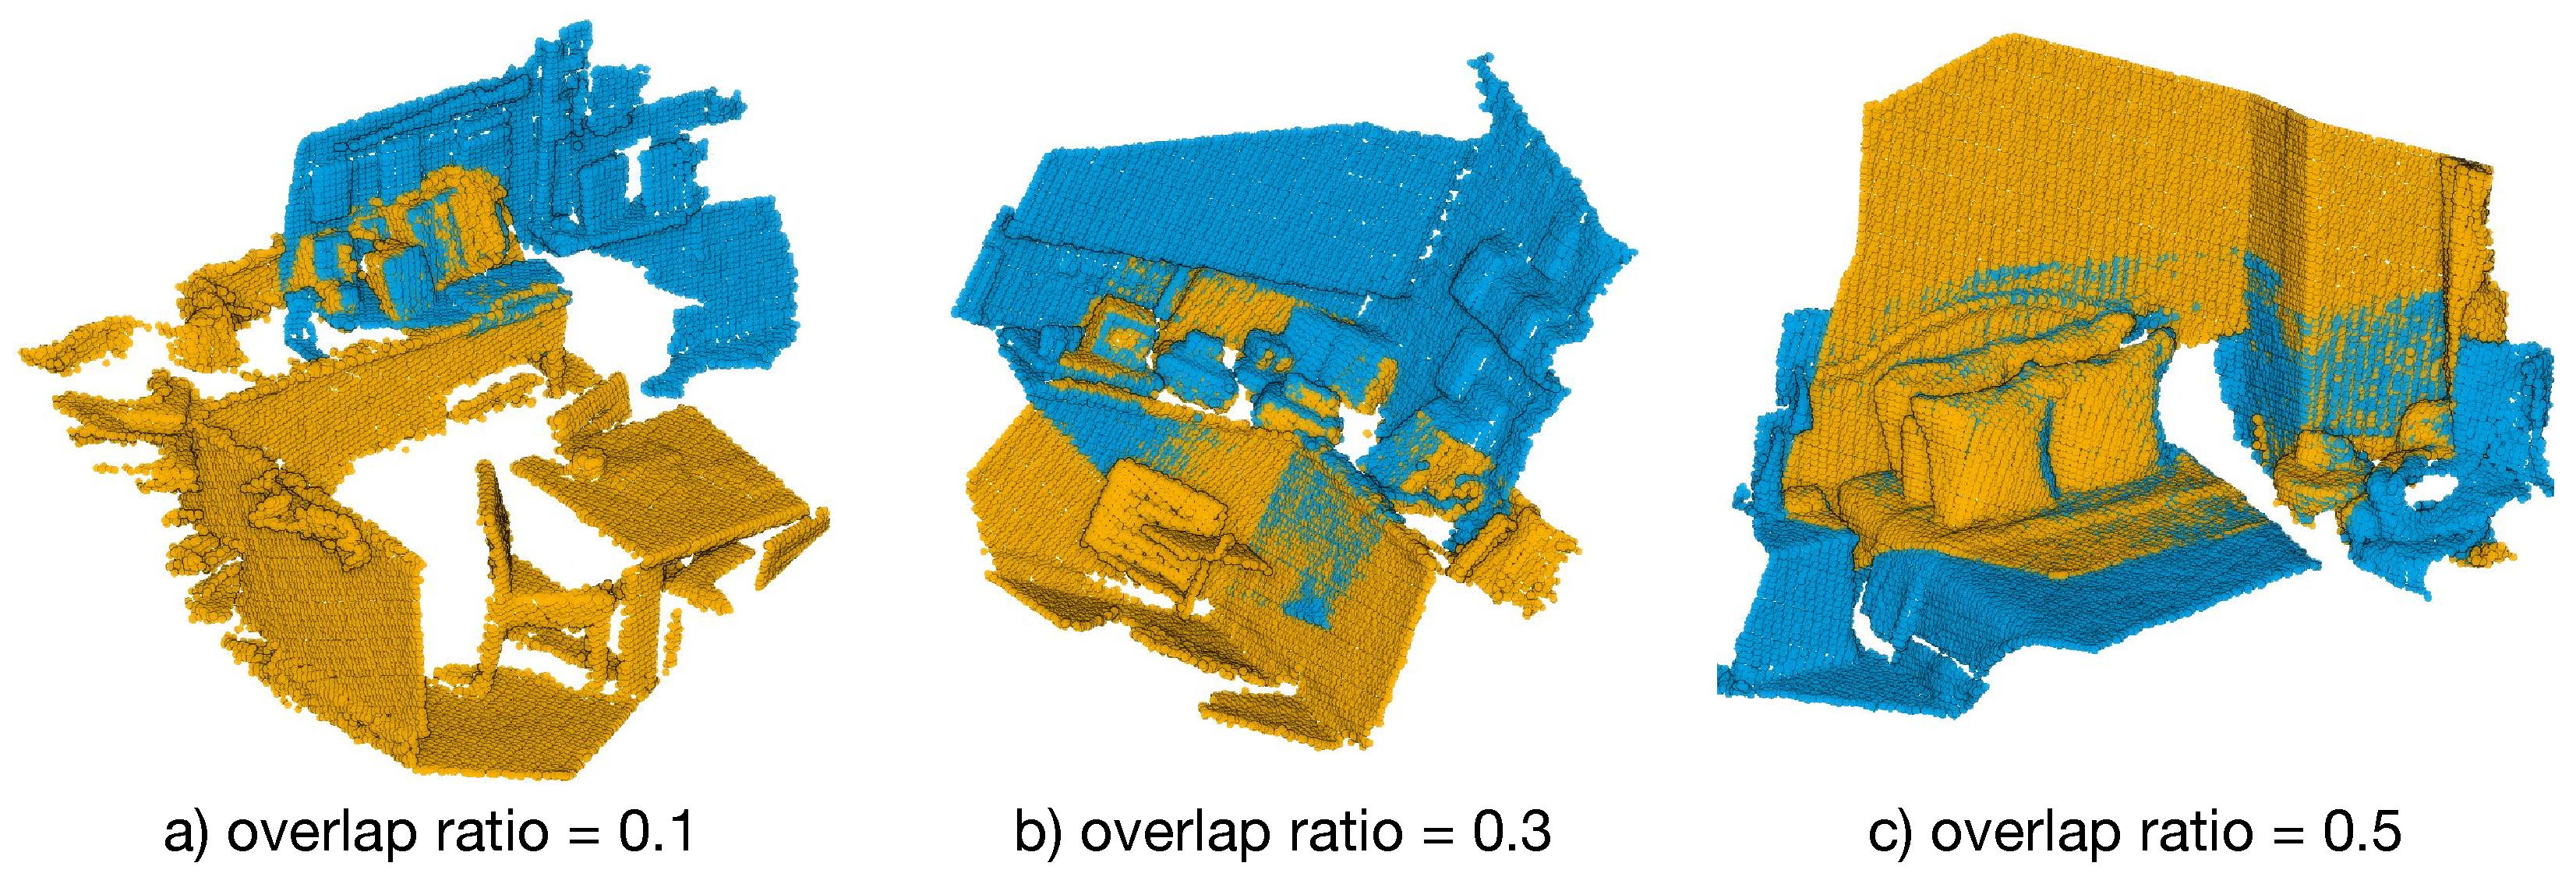
\includegraphics[width=\columnwidth]{figures/images/overlap_samples.pdf}
    \caption{Fragments with different overlap ratios. Overlap is computed relative to the source fragment (orange).}
    \label{fig:demo_overlap}
    
\end{figure}
\subsection{Encoder}
\label{sec:method_encoder}
We follow~\cite{thomas2019kpconv} and first down-sample raw point clouds with a voxel-grid filter of size $V$, such that
$\mathbf{P}$ and $\mathbf{Q}$ have reasonably uniform point density.
In the shared encoder, a series of ResNet-like blocks and strided convolutions aggregate the raw points into \textit{superpoints} $\mathbf{P}'\in\mathbb{R}^{N'\times 3}$ and 
$\mathbf{Q}'\in\mathbb{R}^{M'\times 3}$ with associated features $\mathbf{X}^{\mathbf{P}'} \in \mathbb{R}^{N{'} \times b}$ and $\mathbf{X}^{\mathbf{Q}'} \in \mathbb{R}^{M' \times b}$.
Note that superpoints correspond to a fixed receptive field, so their number depends on the spatial extent of the input point cloud and may be different for the two inputs.

\subsection{Overlap Attention Module}
\label{sec:method_overlap_attention}
So far, the features $\mathbf{X}^{\mathbf{P}'}$, $\mathbf{X}^{\mathbf{Q}'}$ in the bottleneck encode the geometry and context of the two point clouds. But $\mathbf{X}^{\mathbf{P}'}$ has no knowledge of point cloud $\mathbf{Q}$ and vice versa.
In order to reason about their respective overlap regions, some cross-talk is necessary.
We argue that it makes sense to add that cross-talk at the level of superpoints in the bottleneck, just like a human operator will first get a rough overview of the overall shape to determine likely overlap regions, and only after that identifies precise feature points in those regions.

\paragraph{Graph convolutional neural network}
Before connecting the two feature encodings, we first further aggregate and strengthen their contextual relations individually with a graph neural network (GNN)~\cite{wang2019dynamic}.
In the following, we describe the GNN for point cloud $\mathbf{P}'$.
The GNN for $\mathbf{Q}'$ is the same.
First, the superpoints in $\mathbf{P}'$ are linked into a graph in Euclidean space with the $k$-NN method.
Let ${\mathbf{x}}_i \in \mathbb{R}^{b}$ denote the feature encoding of superpoint $\mathbf{p}'_i$, and $(i,j) \in \mathcal{E}$ the graph edge between superpoints $\mathbf{p}_i'$ and $\mathbf{p}_j'$.
The encoder features are then iteratively updated as
\begin{equation}
    \leftidx{^{(k+1)}}{\mathbf{x}}_i = \max_{(i,j)\in\mathcal{E}} h_\theta\big( \mathrm{cat}[\leftidx{^{(k)}}{\mathbf{x}}_i, \leftidx{^{(k)}}{\mathbf{x}}_j - \leftidx{^{(k)}}{\mathbf{x}}_i]\big)\;,
\end{equation}
where $h_\theta(\cdot)$ denotes a linear layer followed by instance normalization~\cite{ulyanov2016instance} and a LeakyReLU activation~\cite{maas2013rectifier}, $\max(\cdot)$ denotes  element-/channel-wise max-pooling, and $\mathrm{cat}[\cdot,\cdot]$ means concatenation. This update is performed twice with separate (not shared) parameters $\theta$, and the final GNN features ${\mathbf{x}}_i^{\mathrm{GNN}} \in \mathbb{R}^{d_b}$ are obtained as
\begin{equation}
    {\mathbf{x}}_i^{\mathrm{GNN}} =  h_\theta(\text{cat}[\leftidx{^{(0)}}{\mathbf{x}}_i, \leftidx{^{(1)}}{\mathbf{x}}_i,
    \leftidx{^{(2)}}{\mathbf{x}}_i])\;.
\end{equation}

\paragraph{Cross-attention block} 
Knowledge about potential overlap regions can only be gained by mixing information about both point clouds. To this end we adopt a cross-attention block~\cite{sarlin2020superglue} based on the message passing formulation~\cite{gilmer2017neural}.
First, each superpoint in $\mathbf{P}'$ is connected to all superpoints in $\mathbf{Q}'$ to form a bipartite graph.
Inspired by the Transformer architecture~\cite{vaswani2017attention}, vector-valued queries $\mathbf{s}_i\!\in\!\mathbb{R}^{b}$ are used to retrieve the values $\mathbf{v}_j\!\in\!\mathbb{R}^{b}$ of other superpoints based on their keys
$\mathbf{k}_j\!\in\!\mathbb{R}^{b}$, where 
\begin{equation}
    \mathbf{k}_j = \mathbf{W}_k\mathbf{x}_j^{\mathrm{GNN}}\quad
    \mathbf{v}_j = \mathbf{W}_v\mathbf{x}_j^{\mathrm{GNN}}\quad
    \mathbf{s}_i = \mathbf{W}_s\mathbf{x}_i^{\mathrm{GNN}}\\
\end{equation}
and $\mathbf{W}_k$, $\mathbf{W}_v$, and $\mathbf{W}_s$ are learnable weight matrices.
The messages are computed as weighted averages of the values,
\begin{equation}
    \mathbf{m}_{i\leftarrow} = \sum_{j:(i,j)\in\mathcal{E}}a_{ij}\mathbf{v}_j\;,
\end{equation}
with attention weights $a_{ij} = \text{softmax}(\mathbf{s}^{T}_i\mathbf{k}_j / \sqrt{b})$~\cite{sarlin2020superglue}.
I.e., to update a superpoint $\mathbf{p}_i'$ one combines that point's query with the keys and values of all superpoints $\mathbf{q}_j'$.
In line with the literature, in practice we use a multi-attention layer with four parallel attention heads
~\cite{vaswani2017attention}.
The co-contextual features are computed as
\begin{equation}
    \mathbf{x}_i^{\text{CA}} = \mathbf{x}_i^{\mathrm{GNN}} + \mathrm{MLP}(\mathrm{cat}[\mathbf{s}_i, \mathbf{m}_{i\leftarrow}])\;,
\end{equation}
with $\mathrm{MLP}(\cdot)$ denoting a three-layer fully connected network with instance normalization~\cite{ulyanov2016instance} and ReLU~\cite{nair2010rectified} activations after the first two layers.
The same cross-attention block is also applied in reverse direction, so that information flows in both directions, $\mathbf{P}'\!\rightarrow\!\mathbf{Q}'$ and $\mathbf{Q}'\!\rightarrow\!\mathbf{P}'$.

\paragraph{Overlap scores of the bottleneck points}
The above update with co-contextual information is done for each superpoint in isolation, without considering the local context within each point cloud.
We therefore, explicitly update the local context after the cross-attention block using another GNN that has the same architecture and underlying graph (within-point cloud links) as above, but separate parameters $\theta$.
This yields the final latent feature encodings  $\mathbf{F}^{\mathbf{P}'}\!\!\in\!\mathbb{R}^{N'\!\times b}$ and $\mathbf{F}^{\mathbf{Q}'}\!\!\in\!\mathbb{R}^{M'\!\times b}$, which are now conditioned on the features of the respective other point cloud.
Those features are linearly projected to overlap scores $\mathbf{o}^{\mathbf{P}'}\!\!\in\!\mathbb{R}^{N'}$ and $\mathbf{o}^{\mathbf{Q}'}\!\!\in\!\mathbb{R}^{M'}$, which can be interpreted as probabilities that a certain superpoint lies in the overlap region.
Additionally, one can compute \emph{soft correspondences} between superpoints and from the correspondence weights predict the \emph{cross-overlap score} of a superpoint $\mathbf{p}'_i$, i.e., the probability that its
correspondence in $\mathbf{Q}'$ lies in the overlap region:
\begin{equation}
    \tilde{o}_i^{\mathbf{P}'}:= \mathbf{w}_i^{T} \mathbf{o}^{\mathbf{Q}'}, \quad w_{ij} := \mathrm{softmax}\big(\frac{1}{t}\langle\mathbf{f}^{\mathbf{P}'}_i, \mathbf{f}^{\mathbf{Q}'}_j\rangle\big)\;,
    \label{eq:softass}
\end{equation}
where $\langle \cdot,\cdot \rangle$ is the inner product, and $t$ is the temperature parameter that controls the soft assignment. In the limit $t\!\rightarrow\!0$, Eq.~\eqref{eq:softass} converges to hard nearest-neighbour assignment.






\subsection{Decoder}
\label{sec:method_decoder}
Our decoder starts from conditioned features $\mathbf{F}^{\mathbf{P}'}$, concatenates them with the overlap scores $\mathbf{o}^{\mathbf{P}'}$, $\tilde{\mathbf{o}}^{\mathbf{P}'}$, and outputs per-point feature descriptors $\mathbf{F}^{\mathbf{P}}\!\!\in\!\mathbb{R}^{N\times32}$ and refined per-point overlap and matchability scores $\mathbf{o}^{\mathbf{P}},\mathbf{m}^{\mathbf{P}}\!\in \!\mathbb{R}^{N}$.
The matchability can be seen as a "conditional saliency" that quantifies how likely a point is to be matched correctly, given the points (resp.\ features) in the other point cloud $\mathbf{Q}$.

The decoder architecture combines {NN}-upsampling with linear layers, and includes skip connections from the corresponding encoder layers.
We deliberately keep the overlap score and the matchability separate
to disentangle the reasons why a point is a good/bad candidate for matching: in principle a point can be unambiguously matchable but lie outside the overlap region, or it can lie in the overlap but have an ambiguous descriptor.
Empirically, we find that the network learns to predict high matchability mostly for points in the overlap; probably reflecting the fact that the ground truth correspondences used for training, naturally, always lie in the overlap.
For further details about the architecture, please refer to Appendix and the \href{https://github.com/ShengyuH/OverlapPredator}{source code}.

\subsection{Loss Function and Training}
\label{sec:method_training}
\acro\ is trained end-to-end, using three losses \wrt ground truth correspondences as supervision.

\paragraph{Circle loss}
To supervise the point-wise feature descriptors we follow%
\footnote{Added to the repository after publication, not mentioned in the paper.}%
~\cite{bai2020d3feat} and use the circle loss~\cite{sun2020circle}, a variant of the more common triplet loss.
Consider again a pair of overlapping point clouds $\mathbf{P}$ and $\mathbf{Q}$, this time aligned with the ground truth transformation. We start by extracting the points $\mathbf{p}_i\!\in\!\mathbf{P}_p\!\subset\!\mathbf{P}$ that have at least one (possibly multiple) correspondence in $\mathbf{Q}$,
where the set of correspondences $\mathcal{E}_p(\mathbf{p}_i)$  is defined as points in $\mathbf{Q}$ that lie within a radius $r_p$ around $\mathbf{p}_i$. Similarly, all points of $\mathbf{Q}$  outside a (larger) radius
$r_s$ form the set of negatives $\mathcal{E}_n(\mathbf{p}_i)$.
The circle loss is then computed from $n_p$ points sampled randomly from $\mathbf{P}_p$: %
\begin{equation}
\mathcal{L}_c^\mathbf{P} = \frac{1}{n_p}\sum\limits_{i=1}^{n_p} \log \Big [ 1 +\!\! \sum\limits_{j\in\mathcal{E}_p}\!e^{ \beta_p^j(d_i^j - \Delta_p)} \cdot\!
\sum\limits_{k\in\mathcal{E}_n} \!e^{\beta_n^k(\Delta_n - d_i^k)}\Big ],
\end{equation}
where $d_i^j=||\mathbf{f}_{\mathbf{p}_i} - \mathbf{f}_{\mathbf{q}_j} ||_2$ denotes distance in feature space, and $\Delta_n,\Delta_p$ are negative and positive margins, respectively. The weights $\beta_p^j\!=\!\gamma(d_i^j\!-\!\Delta_p)$ and $\beta_n^k\!=\!\gamma(\Delta_n\!-\!d_i^k)$ are determined individually for each positive and negative example, using the empirical margins $\Delta_p\!:=\!0.1$ and $\Delta_n\!:=\!1.4$ with hyper-parameter $\gamma$. The reverse loss  $\mathcal{L}_c^\mathbf{Q}$ is computed in the same way, for a total circle loss $\mathcal{L}_c = \frac{1}{2}(\mathcal{L}_c^\mathbf{P} + \mathcal{L}_c^\mathbf{Q})$.

\paragraph{Overlap loss}
The estimation of the overlap probability is cast as binary classification and supervised using the overlap loss $\mathcal{L}_o\!=\!\frac{1}{2} (\mathcal{L}^\mathbf{P}_o + \mathcal{L}^\mathbf{Q}_o)$, where 
\begin{equation}
\mathcal{L}^\mathbf{P}_o = \frac{1}{|\mathbf{P}|} \sum_{i=1}^{|\mathbf{P}|} \overbar{o}_{\mathbf{p}_i}\log(o_{\mathbf{p}_i}) + (1 - \overbar{o}_{\mathbf{p}_i})\log(1 - o_{\mathbf{p}_i}).
\end{equation}
The ground truth label $\overbar{o}_{\mathbf{p}_i}$ of point $\mathbf{p}_i$ is defined as
\begin{equation}
    \overbar{o}_{\mathbf{p}_i} =     
    \begin{cases}
      1, & ||\overbar{\mathbf{T}}_\mathbf{P}^\mathbf{Q}(\mathbf{p}_i) - \mathsf{NN}(\overbar{\mathbf{T}}_\mathbf{P}^\mathbf{Q}(\mathbf{p}_i),\mathbf{Q}) ||_2 < r_o \\
      0, & \text{otherwise}
    \end{cases},
\end{equation}
with overlap threshold $r_o$. The reverse loss $\mathcal{L}_o^\mathbf{Q}$ is computed in the same way.
The contributions from positive and negative examples are balanced with weights inversely proportional to their relative frequencies.

\paragraph{Matchability loss}
Supervising the matchability scores is more difficult, as it is not clear in advance which are the right points to take into account during correspondence search.
We follow a simple intuition: good keypoints are those that can be matched successfully at a given point during training, with the current feature descriptors.
Hence, we cast the prediction as binary classification and generate the ground truth labels on the fly.
Again, we sum the two symmetric losses, $\mathcal{L}_m = \frac{1}{2} (\mathcal{L}^\mathbf{P}_m + \mathcal{L}^\mathbf{Q}_m)$, with
\begin{equation}
\mathcal{L}^\mathbf{P}_m\!= \frac{1}{|\mathbf{P}|} \sum_{i=1}^{|\mathbf{P}|} \overbar{m}_{\mathbf{p}_i}\log(m_{\mathbf{p}_i})+(1-\overbar{m}_{\mathbf{p}_i})\log(1-m_{\mathbf{p}_i}),
\end{equation}
where ground truth labels $\overbar{m}_{\mathbf{p}_i}$ are computed on the fly via nearest neighbour search $\mathsf{NN}_\mathbf{F}(\cdot,\cdot)$ in feature space:
\begin{equation}
    \overbar{m}_{\mathbf{p}_i}\!=     
    \begin{cases}
      1, & ||\overbar{\mathbf{T}}_\mathbf{P}^\mathbf{Q}(\mathbf{p}_i)\!-\!\mathsf{NN}_\mathbf{F}(\mathbf{p}_i,\mathbf{Q}) ||_2\!<\!r_m \\
      0, & \text{otherwise}.
    \end{cases}
\end{equation} 

\begin{figure}[t]
    \centering
    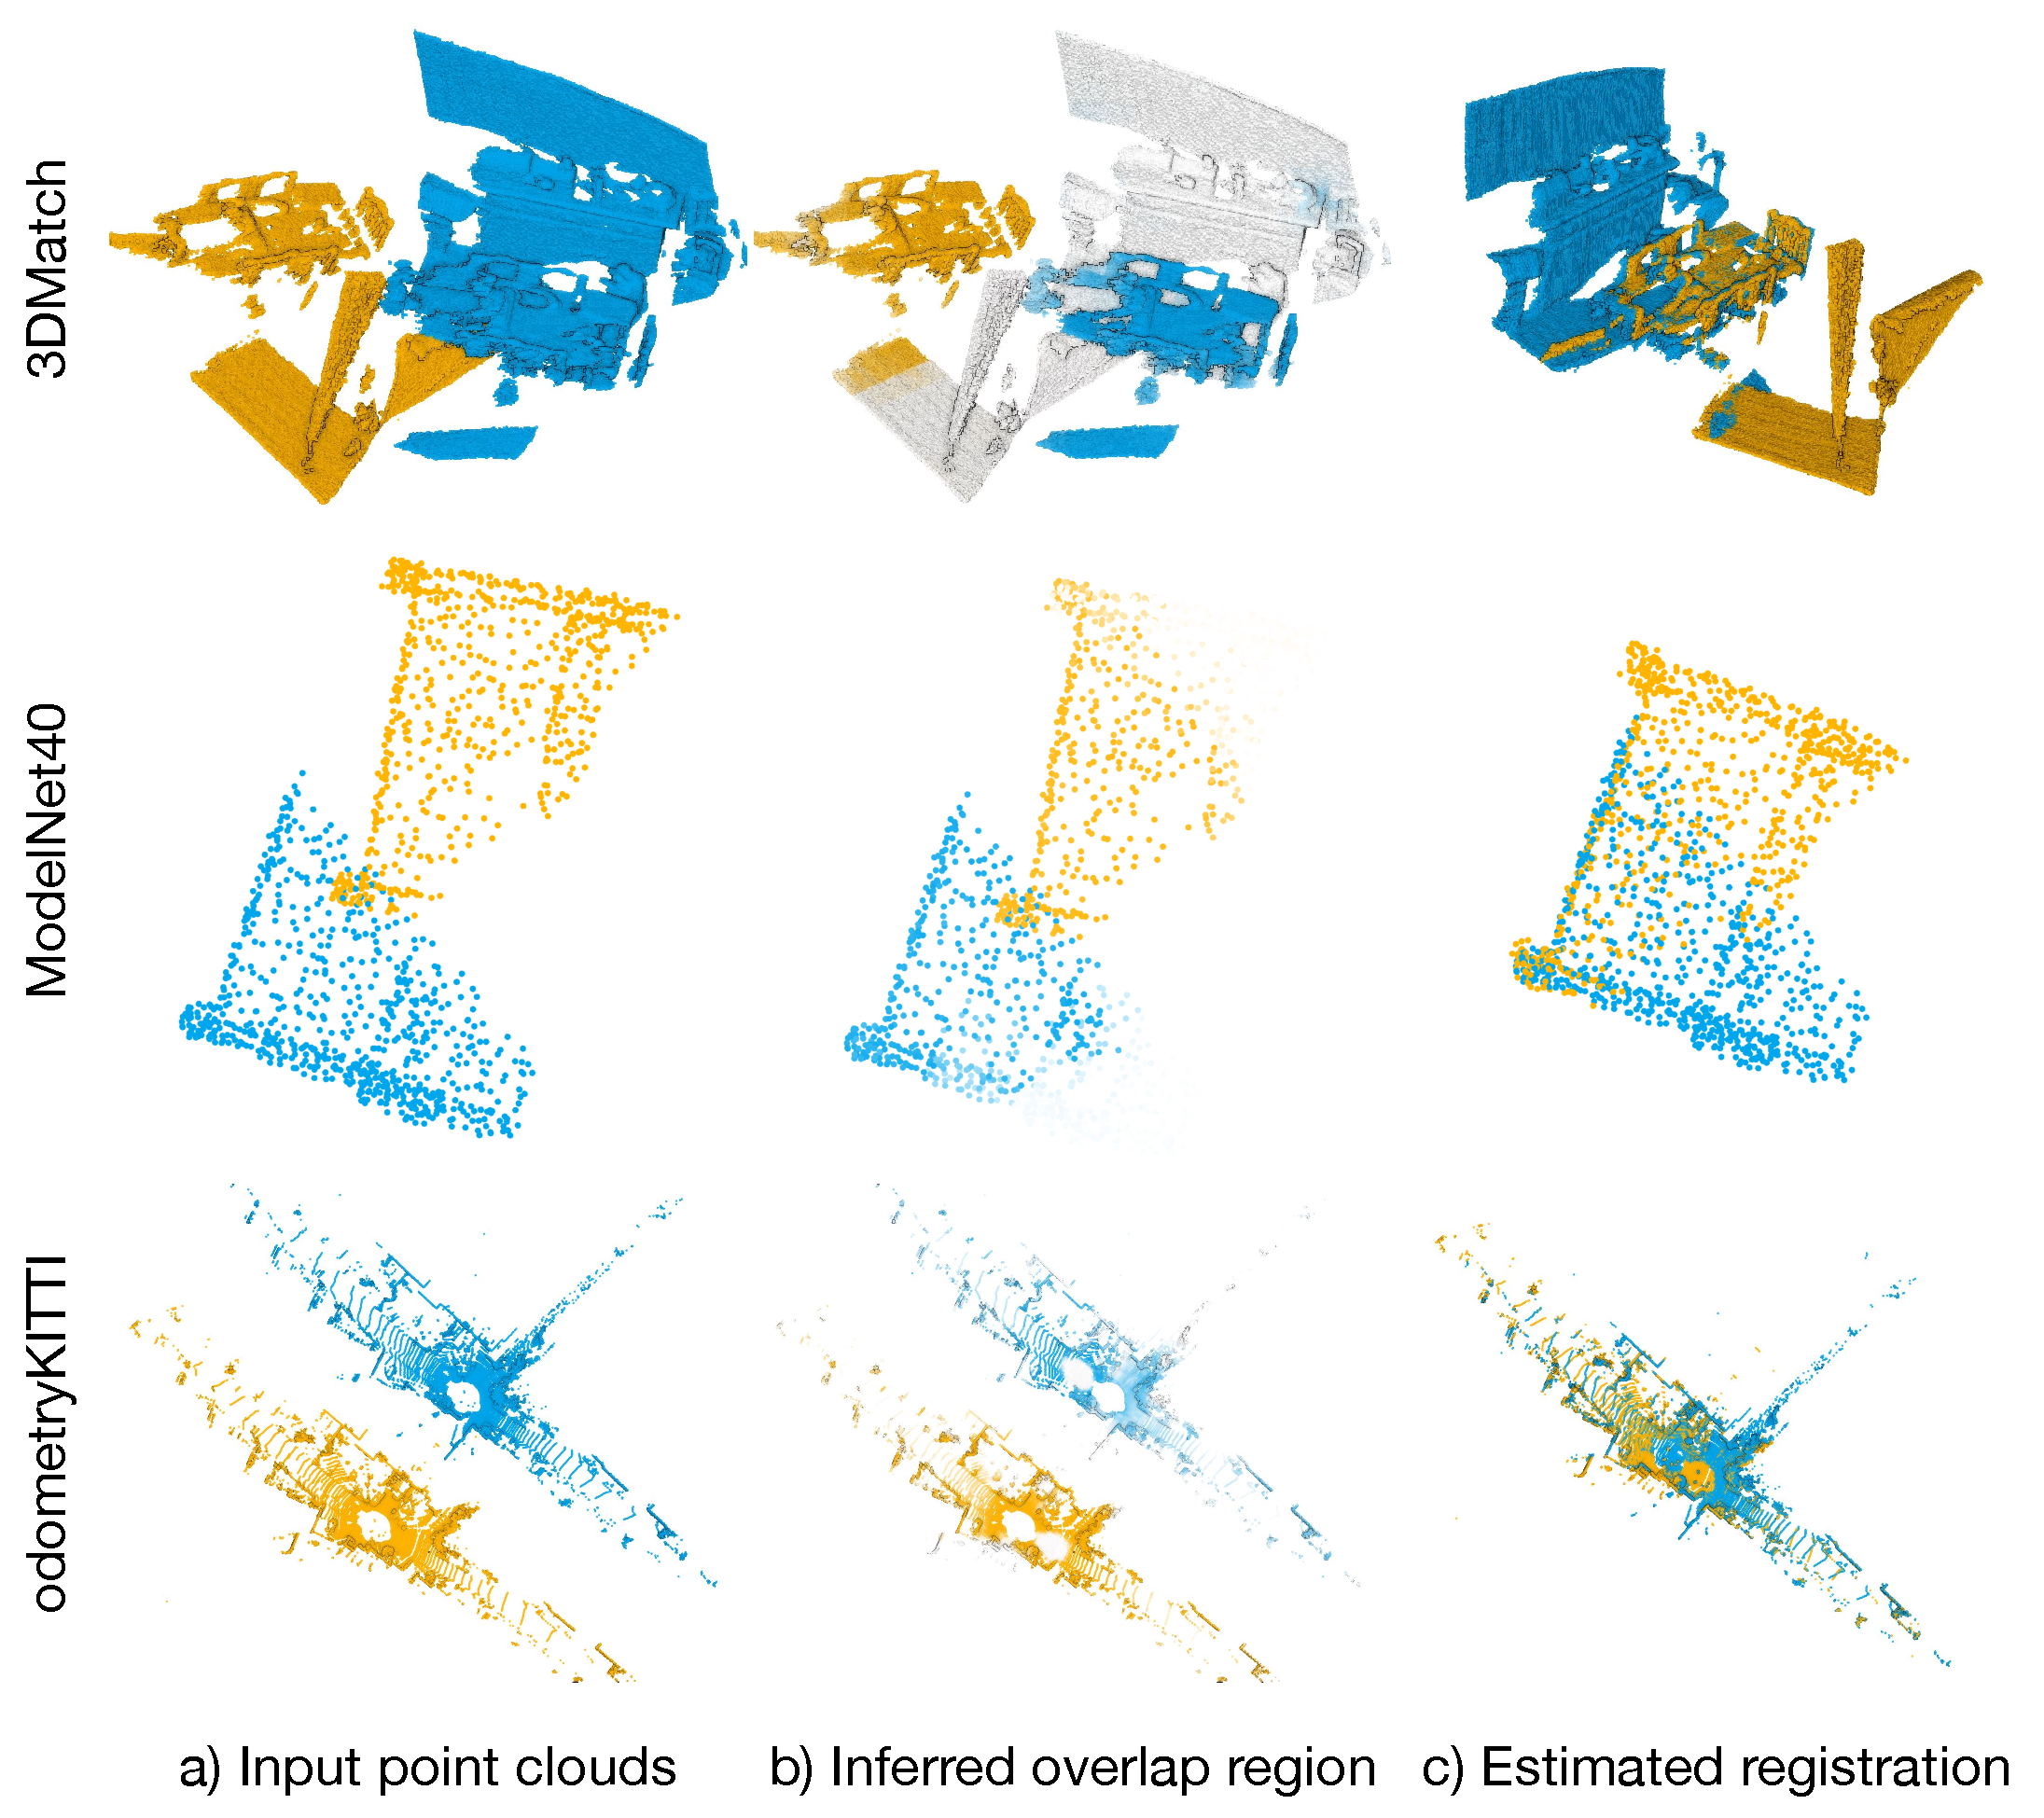
\includegraphics[width=1.0\columnwidth]{figures/images/qualitative_all.pdf}
    \caption{Example results of \acro\ that succeeds in attending to the overlap region to enable robust registration.}
    \label{fig:3DMatch_qualitative}
\end{figure}

\paragraph{Implementation and training}
\acro\ is implemented in pytorch and can be trained on a single RTX 3090 GPU. At the start of the training we supervise \acro\ only with the circle and overlap losses, the matchability loss is added only after few epochs, when the point-wise features are already meaningful (i.e., $>$30\% of interest points can be matched correctly).
The three loss terms are weighted equally. For more details, please refer to Appendix.